% !TeX encoding = UTF-8
% !TeX program = pdflatex
% !TeX spellcheck = en_US
\documentclass[binding=0.6cm]{sapthesis}
\usepackage{microtype}
\usepackage[english]{babel}
\usepackage[utf8]{inputenc}
\usepackage{csquotes}

%\usepackage{setspace}
%\singlespacing
%\linespread{0.9}
%\usepackage[backend=bibtex,citestyle=authoryear,bibstyle=apa]{biblatex}
\usepackage[backend=biber,style=apa]{biblatex}
\bibliography{bibliography}

%%%% ZAVVE: to add parenthesis to \cite{} command
\newcommand{\mycite}[1]{(\cite{#1})}

\usepackage{hyperref}
\hypersetup{
    %hyperfootnotes=true,			
    %bookmarks=true,			
    %colorlinks=true,
    %linkcolor=red,
    %linktoc=page,
    %anchorcolor=black,
    %citecolor=red,
    %urlcolor=blue,
    pdftitle={Parametrized CF Explanations in Graph Neural Networks},
    pdfauthor={Giammarco D'Alessandro},
    pdfkeywords={thesis, sapienza, roma, university}
 }


\title{Parametrized Counterfactual Explanations for Node Classification in Graph Neural Networks}
\author{Giammarco D'Alessandro}
\IDnumber{1753102}
\course{Corso di laurea magistrale in Engineering in Computer Science - Ingegneria Informatica}
\courseorganizer{Facoltà di Ingengneria dell'Informazione, Informatica e Statistica}
\AcademicYear{2022/2023}
\advisor{Prof. Fabrizio Silvestri}
\coadvisor{Prof. Simone Scardapane}
%\examdate{... November 2023}
\authoremail{dalessandro.1753102@studenti.uniroma1.it}
\copyyear{2023}
%\thesistype{Master thesis}

\begin{document}

\frontmatter
\maketitle
\dedication{Dedicato a\\Fulmine di Pegasus}

%%%% ZAVVE: to increase page headline space
%\setlength{\headheight}{35pt}.
%\setlength{\headsep}{12pt}.

\begin{abstract}
Given the increasing popularity of Graph Neural Networks (GNNs) in real-world applications such as computational biology, natural language processing (NLP), and computer security, etc...; and the \textit{black-box} nature of such models, several methods have been developed for explaining their predictions. One recent approach to address this problem is counterfactual reasoning, where the goal of an explainer algorithm is to induce a change in the GNN prediction by minimal perturbation of the input structure. 

%Existing methods for interpreting predictions from GNNs have primarily focused on generating subgraphs that are especially relevant for a particular prediction. However, such methods are not counterfactual (CF) in nature: given a prediction, we want to understand how the prediction can be changed in order to achieve an alternative outcome. In this work, we propose a method for generating CF explanations for GNNs: the minimal perturbation to the input (graph) data such that the prediction changes. Using only edge deletions, we find that our method, CF-GNNExplainer, can generate CF explanations for the majority of instances across three widely used datasets for GNN explanations, while removing less than 3 edges on average, with at least 94\% accuracy. This indicates that CF-GNNExplainer primarily removes edges that are crucial for the original predictions, resulting in minimal CF explanations.

%Graph neural networks (GNNs) find applications in various domains such as computational biology, natural language processing, and computer security. Owing to their popularity, there is an increasing need to explain GNN predictions since GNNs are black-box machine learning models. One way to address this is counterfactual reasoning where the objective is to change the GNN prediction by minimal changes in the input graph. Existing methods for counterfactual explanation of GNNs are limited to instance-specific local reasoning. This approach has two major limitations of not being able to offer global recourse policies and overloading human cognitive ability with too much information. In this work, we study the global explainability of GNNs through global counterfactual reasoning. Specifically, we want to find a small set of representative counterfactual graphs that explains all input graphs. Towards this goal, we propose GCFExplainer, a novel algorithm powered by vertexreinforced random walks on an edit map of graphs with a greedy summary. Extensive experiments on real graph datasets show that the global explanation from GCFExplainer provides important high-level insights of the model behavior and achieves a 46.9% gain in recourse coverage and a 9.5% reduction in recourse cost
\end{abstract}

\tableofcontents
\mainmatter

%%%%%%%%%%%%%%%%%%%%%%%%% CHAP.1 : Introduction 
\chapter{Introduction}
\label{chap:1-intro} 
In recent years, Graph Neural Networks (GNNs) have emerged as a powerful tool for analyzing complex relational data represented in the form of graphs. Graphs are pervasive in various domains, including social networks, biological systems, transportation networks, and recommendation systems. The ability of GNNs to model and understand these graph structures has led to significant advancements in tasks such as node classification, link prediction, and community detection.

Node classification, a fundamental task in graph analysis, involves predicting labels or categories for nodes in a graph based on their structural and attribute information. Despite the remarkable success of GNNs in node classification, interpreting their decisions remains a challenge. Understanding why a GNN predicts a specific label for a node is crucial for building trust, improving model robustness, and gaining insights into the underlying data.

One promising approach to address the interpretability challenge in GNNs is the integration of counterfactual explanations in eXplainable Artificial Intelligence (XAI\footnotemark). Counterfactual explanations provide meaningful insights into model predictions by identifying what changes in the input features would lead to a different prediction. In the context of node classification, counterfactual explanations can elucidate the necessary alterations to the node's attributes or connections that would result in a different predicted label.

\footnotetext{The acronym was made popular by the USA Defense Advanced Research Projects Agency when launching to the research community the challenge of designing self-explanatory AI systems (\url{https://www.darpa.mil/program/explainable-artificial-intelligence}).}


This thesis focuses on the incorporation of counterfactual explanations to enhance interpretability in GNNs for node classification. We explore how these explanations can shed light on the decision-making process of GNNs and provide actionable insights for stakeholders. The objective is to bridge the gap between predictive accuracy and model interpretability, facilitating the deployment of GNNs in real-world applications where transparency and trustworthiness are paramount.

In this introductory chapter, we present an overview of the research problem, define the research objectives, outline the scope and contributions of this thesis, and provide a brief outline of the subsequent chapters. Additionally, we discuss the significance of counterfactual explanations in the context of GNNs and node classification, setting the stage for the subsequent chapters that delve deeper into this research domain.

\section{Thesis outline}
The subsequent chapters of this thesis are organized as follows:
\begin{itemize}
    \item Chapter 2: Background
    \item Chapter 3: CFPG
    \item Chapter 4: Experimental and evaluation
    \item Chapter 5: Conclusions and future work
\end{itemize}


%%%%%%%%%%%%%%%%%%%%%%%%% CHAP.2 : Introduction
\chapter{Background}
\label{chap:2-background}
Background in generale, intro al background

\section{Graph Neural Networks}
\label{sec:bg.gnn}
Graph Neural Networks (GNNs, \cite{gnnModel2009}) represent a revolutionary paradigm in the field of machine learning, particularly suited for analyzing and extracting insights from complex structured data, such as graphs. Traditional neural networks excel at processing signals like images, speech, videos or sequences in which there is an underlying Euclidean structure, but they struggle with non-Euclidean data, like graphs. Such kinds of data implies that there are no such familiar properties as global parameterization, common system of coordinates, vector space structure, or shift-invariance. Consequently, basic operations like convolution that are taken for granted in the Euclidean case are even not well defined on non-Euclidean domains \mycite{Bronstein_2017}. 

Graph Neural Networks, on the other hand, have emerged as a powerful tool for handling these intricate data structures by incorporating graph-related properties. Recent developments have increased their capabilities and expressive power. Practical applications have become popular in a really wide spectrum of different areas such as drug discovery \mycite{doi:10.1021/acs.jmedchem.9b00959}, physics simulations \mycite{sanchezgonzalez2020learning}, fake news detection \mycite{monti2019fake}, recommendation systems \mycite{eksombatchai2017pixie} and many others \mycite{hamilton2020graph}.

In essence, GNNs are a class of deep learning models designed to operate on graphs, capturing both the node-level and the edge-level information within a graph. They are engineered to learn meaningful representations of nodes and edges by leveraging the graph's topology and associated features. These representations can be exploited in performing various tasks, such as node classification, link prediction, community detection, and graph generation. More generally GNNs have shown remarkable performance in domains where relationships and interactions between entities are crucial for understanding system dynamics and making informed predictions.

This introduction will delve deeper into the foundations, architectures, and applications of Graph Neural Networks, providing a comprehensive understanding of this cutting-edge approach to processing complex relational data. First it will go through some basics of graph theory and it will analyze how these concepts can be used to model real world scenarios, and how neural networks  can exploit the information encoded in such models. Last it will added a brief presentation of different types of GNNs and their peculiarities.

\subsection{From graphs to Graph Neural Networks}
\label{sec:bg.gnn.graph-base}

\begin{figure}
    \centering
    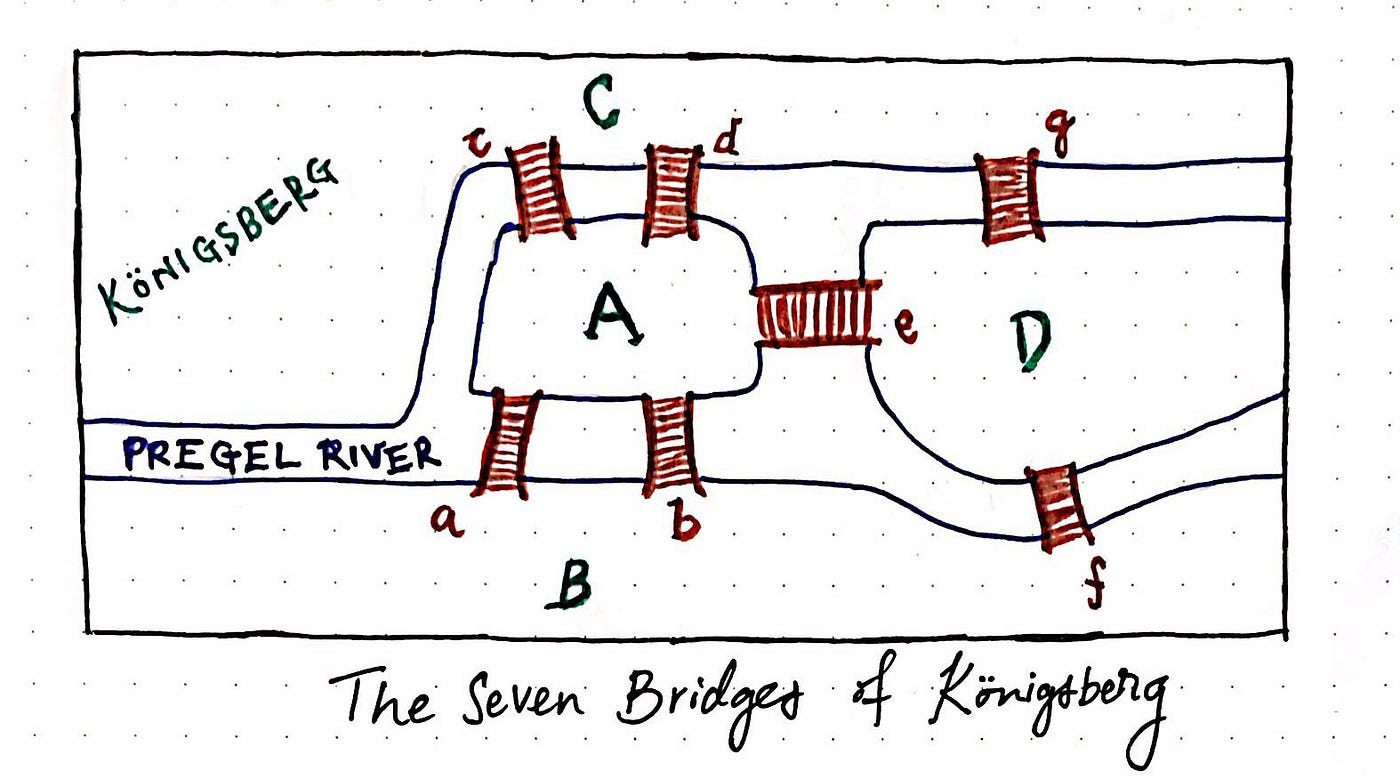
\includegraphics[width=\textwidth]{imgs/background/konigsberg-bridges-02.jpeg}   
    \caption{\textit{A schematic representation of the seven bridges of Königsberg problem, for which Leonhard Euler proposed a negative resolution in his famous 1736 paper, laying the foundation for modern graph theory. The problem was to devise a walk through the city that would cross each of those bridges once and only once.}}
    \label{fig:bg.gnn.konigsbridge}
\end{figure}
The theory of graphs (also graph theory) can be traced back at least to the illustrious swiss mathematician Leonhard Euler, who in a 1736 paper \mycite{gazette_1987} solved a puzzle about an optimal tour of the town of Königsberg (Fig.\ref{fig:bg.gnn.konigsbridge}). Some more developments were made in the $19th$ century, the very term "graph" was introduced in this period by Sylvester in a paper published in 1878 in Nature \mycite{Sylvester1878ChemistryAA}, where he draws an analogy between "quantic invariants" and "co-variants" of algebra and molecular diagrams. The field straight-up exploded during the $20th$ century, the first textbook on graph theory was published in 1936 by Dénes Kőnig, followed by many others \mycite{tutte2001graph}; currently graphs are one of the principal objects of study in discrete mathematics. Graphs, in the realm of mathematics and computer science, are powerful mathematical abstractions used to model relationships between entities. In its basic type, a simple graph G can be defined as the couple:
\begin{equation}
    \label{eq:bg.gnn.graph-def}
    G = (V,E)
\end{equation}
where $V = \{v_1,v_2,...,v_N\}$ is the set of \textit{vertices} or \textit{nodes}, the entities ($N = |V|$), and $E = \{(v_i,v_j) | v_i,v_j \in V; i \ne j\}$ is the set of \textit{edges}, also called links, modeling the relationship between two entities. A basic distinction is made between \textit{undirected} graphs, where edges link two vertices symmetrically, i.e. there is no difference between the edges $(v_i,v_j)$ and $(v_j,v_i)$; and \textit{directed} graphs, where edges link two vertices asymmetrically, thus $(v_i,v_j)$ and $(v_j,v_i)$ would be two separated edges \mycite{cormen2022introduction}. Moreover two other categorization are generally made: considering the types of its components and their behavior  over time. 
A graph can be \textit{homogeneous}, when nodes and edges of the graph have all the same type; or \textit{heterogeneous} when nodes and edges are associated with different types. More specifically, in a heterogeneous graph $(V, E, \phi, \psi)$, each node $v_i$ is associated with a type $\phi(vi)$ and each edge $e_j$ with a type $\psi(ej)$. 
When input features or the topology of the graph vary with time, i.e. the existence of nodes and edges may change at different points in time, the graph is regarded as \textit{dynamic}, otherwise is considered \textit{static}. The time information should be carefully considered in dynamic graphs \mycite{zhou2021graph,wang2021mthetgnn}. Note that these categories are orthogonal, meaning that these properties can be combined in the same graph, e.g. one can deal with a dynamic directed heterogeneous graph.
%%% cyclic/acyclic graph

%%% more detailed examples
%%% immaginie di applicazione grafi in real world
One of the typical application of graphs is modeling the relationships inside social networks \mycite{Wu_Lian_Xu_Wu_Chen_2020}, tools to study patterns in collective behaviour of people, institutions and organizations, where the set of social actors can be represented with the nodes of the graph, and their relative interactions are represented by the edges (e.g. the standard example for a social graph would be a “friendship graph”; here, $V$ is again a set of people and $E$ is the set of $(u, v) \in V$ such that $u$ and $v$ are friends). This perspective on social network provides a set of methods for analyzing the structure of whole social entities as well as a variety of theories explaining the dynamics and patterns observed in these structures \mycite{wasserman_faust_1994}. Even though realities such as social networks can be easily seen as graphs and modeled accordingly this data structures are an extremely powerful and general representation of data, many other domains can actually be modeled as graphs, like images and text. Although counterintuitive, one can learn more about the symmetries and structure of images and text by viewing them as graphs. 
Traditionally, we visualize images as rectangular grids with image channels, often representing them as arrays. However, an alternative way could be seeing images as graphs possessing a regular structure, where each pixel is a node connected to each neighboring pixels through an edge. Specifically, each non-border pixel will maintain precisely 8 neighbors, and the information stored at every node could be a 3-dimensional vector signifying the RGB value of the corresponding pixel. Also text can be easily converted into a graph format by assigning numerical indices to individual characters, words, or tokens, thus creating a sequence of these indices to represent the text. This process yields a straightforward directed graph, where each word or token is a node connected to the succeeding node through an edge. Of course, this is not usually how text and images are encoded: these graph representations are redundant since all images and all text will have very regular structures. In practice, images have a banded structure in their adjacency matrix because all nodes (pixels) are connected in a grid; and the adjacency matrix for text is just a diagonal line, because each word only connects to the prior word, and to the next one, but those trivial examples are supposed to serve as an intuition of how flexible graphs are and how wide can thus be the range of their applications \mycite{distilPub-sanchez-lengeling2021a}.

%%% graph representation, adjacency list/mat ecc...
\subsubsection{Graph representation}
\label{sec:bg.gnn.graph-repr}
Before going into the details of machine learning applied to graphs, we propose here an introduction on how to represent graphs, their components and the relative features. This problem is crucial to encode real world information into graph models and to be able to exploit the complete potentiality of such abstractions in real world applications. Machine learning models typically take rectangular or grid-like arrays as input, more generally we talk about tensors. In mathematics, a tensor is an algebraic object that describes a multilinear relationship between sets of algebraic objects related to a vector space. Tensors may map between different objects such as vectors, scalars, and even other tensors \mycite{Vasilescu2009AM}. In machine learning, tensors have a broader definition and usually refers also to multidimensional arrays, often called informally "data tensors". The rationale behind this representation is that data stored in such a format can be readily fed into any artificial intelligence model based on neural networks, thereby opening up the possibility of analyzing them through a diverse range of algorithms and models. So, it’s not immediately intuitive how to represent graph structured data in a format that is compatible with deep learning.

Graphs can have up to four types of elements that can be potentially useful to perform machine learning tasks: nodes, edges and connectivity. A solution to represent the first two is relatively straightforward. The most common choice to represent nodes is to assign to each node $v$ an index $i$ (e.g. an integer) as an identifier, and a $d$-dimensional vector to encode the node features, so that, in general, we will have a node feature matrix $X$ of dimension ${N \times d}$ grouping all node data. For what concerns edges we can simply follow the definition (Sec.\ref{sec:bg.gnn.graph-base}) identifying each edge $e$ by the couple of nodes it connects in the graph (e.g. if edge $e$ connect nodes $i$ and $j$, we have $e = (v_i,v_j)$) and follow the same idea, if necessary, to encode edge features (in this case the edge feature matrix will have dimension $M \times d$, being $M$ the number of edges) \mycite{cormen2022introduction}. However, representing a graph’s connectivity is more complicated. Several data structures have been proposed to tackle this problem, among them three have resulted to be the most efficient and thus the most used in practice: adjacency matrix, incidence matrix and adjacency list.

The \textit{adjacency matrix} is a two-dimensional tensor ($N \times N$, being $N$ the number of nodes), in which the rows represent source vertices and columns represent destination vertices. Data on edges and vertices must be stored externally. Only the cost for one edge can be stored between each pair of vertices. We note that any two vertices connected by an edges are called adjacent, thus the term \textit{adjacency}. The \textit{incidence matrix} is a two-dimensional tensor ($N \times M$, being $M$ the number of edges), in which the rows represent the vertices and columns represent the edges, so that the entries indicate the incidence relation between the vertex at a row and edge at a column (an edge $e$ is said to be incident to a node $v$, if $e$ is connected to $v$). \textit{Adjacency lists} can be of two types. In one case nodes can be stored as records or objects, and every vertex stores the list of its adjacent vertices. This data structure allows the storage of additional data on the vertices, and even additional data on edges can be stored if they are also stored as objects, in which case each vertex stores its incident edges and each edge stores its incident vertices. The second case is the most common format of \textit{adjacency list}, where all edges are stored together in one single list, which loses the explicit information of the vertices adjacent to a particular node, gaining on efficiency on space usage \mycite{cormen2022introduction}.  

Perhaps, since it can be easily tensorisable the most obvious choice would be to use an adjacency matrix to represent a graph for machine learning purposes. Yet, this particular representation comes with certain limitations. As illustrated by the example dataset table, the quantity of nodes within a real world graph can reach millions, with a highly fluctuating number of edges per node. Consequently, this frequently results in adjacency matrices with significant sparsity, rendering them highly inefficient in terms of space usage. Another big issue is that there can be many adjacency matrices encoding the same connectivity relations (i.e. the same graph), and there could be no guarantee that these different matrices would produce the same result in a deep neural network, that is to say, they are not permutation invariant. The permutation invariance property is a fundamental inductive bias of graph-structured data, resulting in the fact that for a graph with $N$ nodes, there are up to $N!$ different adjacency matrices that are equivalent representations of the same graph. Learning permutation invariant operations is an indipendent area of recent research, we refer the reader to \mycite{mena2018learning,murphy2019janossy} for further details.

There are now dozens (if not hundreds) textbooks available on the subject (\cite{griffin2023applied,cormen2022introduction,diestel2017graph,bondy2011graph,berge1976graphs}; only to cite few relevant ones); we refer the reader to the mentioned books to delve further into the details of all aspects of graph theory given that such a discussion deviates from the main purpose of this background introduction, which is to show the importance of graphs in mathematics, computational sciences and various fields, and why recently a great interest in applying deep learning to these concepts arose. 

%%% ML sui grafi
\subsection{Deep Learning on graphs}
\label{sec:bg.gnn.DL-on-graphs}
Deep learning is part of a broader family of machine learning (ML) methods, mainly based on extracting patterns from raw data using Artificial Neural Networks (ANNs) and representation learning. The adjective "deep" in deep learning refers to learning complicated concepts by building them from simpler ones in a hierarchical or multi-layer manner \mycite{LeCun2015DeepL}. Artificial neural networks are popular realizations of such deep multi-layer hierarchies. In the past few years, the growing computational power of modern GPU-based computers and the availability of large training datasets have allowed successfully training neural networks with many layers and degrees of freedom \mycite{Bronstein_2017}.

\subsubsection{history}
\label{sec:bg.gnn.DL-history}
The history of deep learning can be traced back several decades, with its roots in ANNs and machine learning. In 1943, drawing inspiration from the structure of a biological neuron, Warren McCulloch (a neuroscientist) and Walter Pitts (a logician) proposed a mathematical model of an artificial neuron, providing a foundational concept for the birth of artificial neural networks \mycite{mcculloch-pitts-1943}.   
\begin{figure}
    \footnotesize a)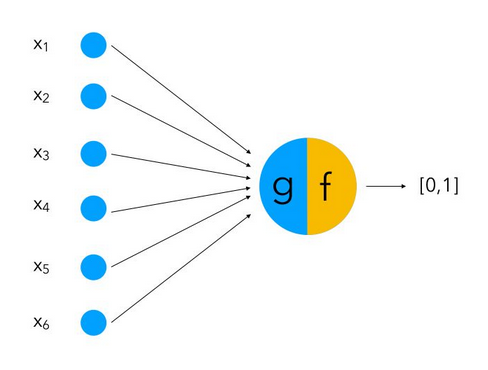
\includegraphics[width=0.45\textwidth]{imgs/background/mcculloch-pitts-02.png} 
    \footnotesize b)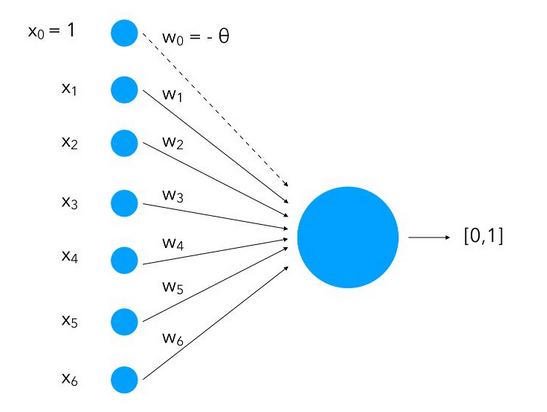
\includegraphics[width=0.45\textwidth]{imgs/background/rosenblatt-02.png} 
    \caption{\textit{On the left (fig.a) a schema of the first artificial neuron introduced by McCulloch and Pitts in 1943. On the right (fig.b) the schema of the perceptron model, introduced by Rosenblatt in 1957.}}
    \label{fig:bg.first-neurons}
\end{figure}
Basically, a neuron in our brain takes an input signal (through the \textit{dendrites}), processes it in its nucleus (\textit{soma}), passes the output through a cable like structure to other connected neurons (\textit{axon} to synapse to another neuron’s dendrites). Although this oversimplification may not align with the biological intricacies of neurons, it offers a high-level representation of how a neuron in our brain functions: receiving input, processing it, and producing an output. This first computational model can be broken down in two parts (Fig.\ref{fig:bg.first-neurons}): the first part, $g$ takes one or more inputs, performs an aggregation and based on the obtained value the second part, $f$ produces an output, i.e. makes a decision. It is following the idea that the interconnection of many simple units, carrying out a simple task, can create the astonishing complexity of human brain that the first artificial neuron was born.

Later on, in 1957, Frank Rosenblatt developed the perceptron, a single-layer neural network capable of binary classification \mycite{rosenblatt-1958-perceptron}.  It was designed to overcome most issues of the McCulloch-Pitts neuron: it can process non-boolean inputs and it can assign different weights to each input automatically; the threshold $\Theta$ is computed automatically. It gained attention for its potential in pattern recognition tasks. The version of Perceptron we use nowadays as standard artificial neuron was introduced in 1969 by Minsky and Papert. Their book criticized the limitations of perceptrons and brought a major improvement to the previous model adding an activation function after the in put aggregation step. The activation function might take several forms and should restrict the weighted sum into a smaller set of possible values that allows a better classification of the output \cite{minsky-papert-1969-perceptrons}. It’s a smoother version than the thresholding applied before. The first comprehensive learning algorithm for supervised, deep, feedforward, multilayer perceptrons was introduced in 1967 by Alexey Ivakhnenko and Lapa \mycite{Ivakhnenko1967CyberneticsAF}.  In a subsequent 1971 paper, they described a deep network with eight layers trained by the group method of data handling. 

In 1989, the book "Parallel Distributed Processing" by Rumelhart, Hinton, and Williams popularized the backpropagation algorithm reviving the interest in the possibility of an efficient training for deep neural networks, and posed the basis for all modern neural network based ML algorithms \mycite{rumelhart-hinton-1989}. One of the first big result that draw attention to deep networks was AlexNet \mycite{krizhevsky2012-nips}, a deep Convolutional Neural Network (CNN) developed by Alex Krizhevsky, that won the ImageNet competition, marking a significant breakthrough and initiating a surge of interest in deep learning. AlexNet competed in the ILSVRC \mycite{ILSVRC15} on September 30, 2012. The deep network achieved a top-5 error of $15.3\%$, more than $10.8$ percentage points lower than that of the runner up. 

In recent years, since the growing availability of GPU processing, deep neural networks have been able to achieve outstanding results in many areas related to Machine Learning. In 2014 Ian Goodfellow introduced Generative Adversarial Networks (GANs), a powerful tool for deep generation of data \mycite{goodfellow2014-GANs}; in the same year DL also made strides in reinforcement learning (a sub-field of ML), with models like Deep Q Networks (DQN) \mycite{Mnih2015-HumanlevelCT}, showing more of the potentiality of deep networks with respect to shallow ones. Another important step forward was made with the introduction of the Transformer architecture, in the 2017 paper "Attention is All You Need" \mycite{vaswani2017-attention} revolutionized natural language processing (NLP), the interdisciplinary sub-field of computer science and linguistics primarily concerned with giving computers the ability to support and manipulate natural language and speech. This led to an important breakthrough in NLP, and in the whole AI spectrum, when the language model BERT (Bidirectional Encoder Representations from Transformers) came out. Being one of the first language model based on trasformers, BERT achieved state-of-the-art results in various NLP tasks thanks to the fact that its the pre-trained model can be fine-tuned with just one additional output layer to create state-of-the-art models for a wide range of applications, such as question answering and language inference, without substantial task-specific architecture modifications.  \mycite{devlin2018-bert}.


\subsubsection{Geometric Deep Learning}
\label{sec:bg.gnn.geo-deep-learning}
Geometric deep learning is an umbrella term for emerging techniques attempting to generalize (structured) deep neural models to non-Euclidean domains such as graphs and manifolds. 

As a unique non-Euclidean data structure for machine learning, graph analysis focuses on tasks such as graph classification, node classification, link prediction, and clustering. 

For nearly two millenia since Euclid’s Elements, the word ‘geometry’ has been synonymous with Euclidean geometry, as no other types of geometry existed. Euclid’s monopoly came to an end in the nineteenth century, with examples of non-Euclidean geometries constructed by Lobachevesky, Bolyai, Gauss, and Riemann. Towards the end of that century, these studies had diverged into disparate fields, with mathematicians and philosophers debating the validity of and relations between these geometries as well as the nature of the “one true geometry”.

According to a popular belief, the Erlangen Programme was delivered in Klein’s inaugural address in October 1872. Klein indeed gave such a talk (though on December 7 of the same year), but it was for a non-mathematical audience and concerned primarily his ideas of mathematical education. What is now called the ‘Erlangen Programme’ was actually a research prospectus brochure \textit{Vergleichende Betrachtungen über neuere geometrische Forschungen} (“A comparative review of recent researches in geometry”) he prepared as part of his professor appointment. See Tobies (2019).


\paragraph{CNN}
\label{sec:bg.gnn.cnn}
\paragraph{Group equivariant CNN}
\label{sec:bg.gnn.geCNN}

Graph Neural Networks (GNNs) represent a category of deep learning techniques tailored for processing graph data. Their impressive performance has propelled these deep learning models to the forefront of widely utilized methods in graph analysis today. 

The first motivation of GNNs is rooted in the long-standing history of neural networks for graphs. In the nineties, Recursive Neural Networks are first utilized on directed acyclic graphs (\cite{Sperduti1997,Frasconi1998}). Afterwards, Recurrent Neural Networks and Feedforward Neural Networks are introduced into this literature respectively in (\cite{gnnModel2009}) and (\cite{Micheli2009}) to tackle cycles. Although being successful, the universal idea behind these methods is building state transition systems on graphs and iterate until convergence, which constrained the extendability and representation ability. Recent advancement of deep neural networks, especially convolutional neural networks (CNNs) result in the rediscovery of GNNs. 

%%% representation learning 
Representation Learning, which is the task of learning representations for complex structured data, is quite challenging with non-euclidean ones. In the last decade, many successful models have been developed for certain kinds of structured data, including data defined on a discretized Euclidean domain. For instance, sequential data, such as text or videos, can be modelled via recurrent neural networks \mycite{TEAlab2018334}, which can capture sequential information, yielding efficient representations as measured on machine translation and speech recognition tasks. Another example are Convolutional Neural Networks (CNNs)\mycite{Lecun1998cnn} have been successfully applied to tackle problems such as image classification (\cite{venkatesan2017convolutional}), semantic segmentation (\cite{jégou2017layers}) or machine translation (\cite{gehring2017convolutional}), where the underlying data representation has a grid-like structure. These architectures efficiently reuse their local filters, with learnable parameters, by applying them to all the input positions \mycite{LeCun2015DeepL}. However these major successes have been restricted to particular types of data that have a simple relational structure (e.g. sequential data, or data following regular patterns), many interesting tasks involve data that can not be represented in a grid-like structure and that instead lies in an irregular domain. This is the case of a large number of systems across various areas including natural science (physical systems (\cite{pmlr-v80-sanchez-gonzalez18a}), social science (social networks as in the example in Sec.\ref{sec:bg.gnn.graph-base}), protein-protein interaction networks (\cite{nips2017_PPI}), knowledge graphs (\cite{ijcai2017p250}) and many other research areas (\cite{nips2017_combOpt}), to name a few. Such data can usually be represented in the form of graphs \mycite{veličković2018gat}.

%Machine learning with graphs blends the line between this distinction because of two key differences in approaching the problem.

\subsection{GNNs}
\label{sec:bg.gnn.gnns}
Graph Neural Networks (GNNs) have been introduced in \mycite{Gori2005graphDomain,gnnModel2009} as a generalization of recursive neural networks that can directly deal with a more general class of graphs, e.g. cyclic, directed and undirected graphs. The fundamental principle behind GNNs is to produce representations of graph (and/or its components) that can be used in downstream tasks such as graph or node classification.

This first step of GNN design, usually called Graph Representation Learning (GRL) aim at learning low-dimensional continuous vector representations for graph-structured data, also called embeddings. Broadly speaking, GRL can be divided into two classes of learning problems, unsupervised and supervised (or semi-supervised) GRL. The first family aims at learning low-dimensional Euclidean representations that preserve the structure of an input graph. The second family also learns low-dimensional Euclidean representations but for a specific downstream prediction task such as node or graph classification. Different from the unsupervised setting where inputs are usually graph structures, in supervised settings inputs are usually composed of different signals defined on graphs, commonly known as node or edge features.

\begin{figure}
    \label{fig:bg.graph_repr}
    \centering
    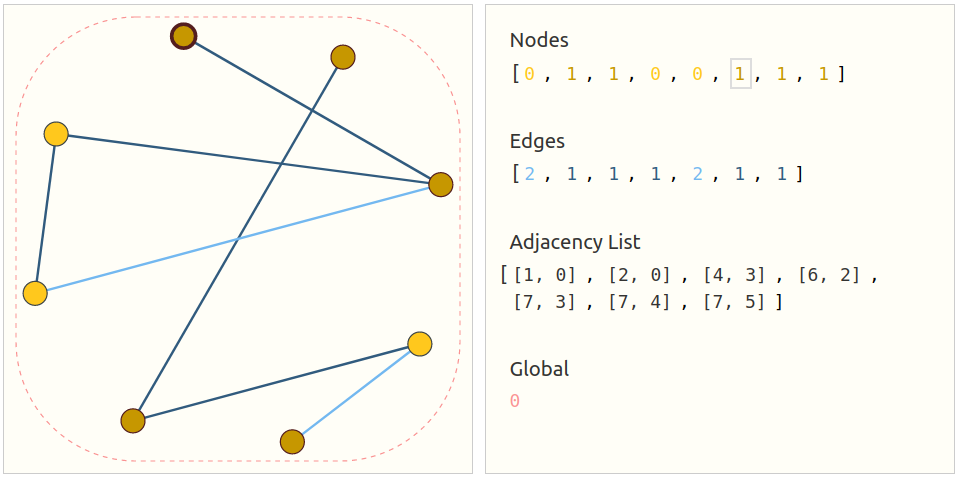
\includegraphics[width=\textwidth]{imgs/background/graph-repr.png}   
    \caption{the dataset format, one json row}
\end{figure}

It should be noted that the figure uses scalar values per node/edge/global, but most practical tensor representations have vectors per graph attribute. Instead of a node tensor of size [nnodes] we will be dealing with node tensors of size [nnodes,nodedim]. Same for the other graph attributes.


GNNs consist of an iterative process, which propagates the node states until equilibrium; followed by a neural network, which produces an output for each node based on its state. This idea was adopted and improved by Li et al. (2016), which propose to use gated recurrent units (Cho et al., 2014) in the propagation step.

Having introduced the basic concepts around graphs, to better better comprehend their success we present an overview of the principal tasks that can be performed through graph representation. There are three general types of prediction tasks on graphs:
\begin{itemize}
    \item In a graph-level task, our goal is to predict the property of an entire graph.
    \item For a node-level task, we predict some property for each node in a graph. 
    \item For an edge-level task, we want to predict the property or presence of edges in a graph.
\end{itemize}

For example, for a molecule represented as a graph, we might want to predict what the molecule smells like, or whether it will bind to a receptor implicated in a disease. This is analogous to image classification problems with MNIST and CIFAR,  where we want to associate a label to an entire image. With text, a similar problem is sentiment analysis where we want to identify the mood  r emotion of an entire sentence at once.

For the three levels of prediction problems described above (graph-level, node-level, and edge-level), we will show that all of the following problems can be solved with a single model class, the GNN. But first, let’s take a tour through the three classes of graph prediction problems in more detail, and provide concrete examples of each.


\subsection{Pooling and message passing}
\label{sec:bg.gnn.pool-message}
\subsection{GNNs architectures}
\label{sec:bg.gnn.gnn-archs}

\section{Explainability - XAI}
\label{sec:bg.xai}
Explainable Artificial Intelligence (XAI) stands at the forefront of the evolving field of artificial intelligence (AI) and seeks to bridge the gap between advanced AI models and human comprehension. As AI systems become increasingly sophisticated and pervasive in our lives, understanding their decision-making processes and outcomes is crucial for fostering trust, transparency, and usability. XAI aims to unravel the 'black box' nature of complex AI algorithms, providing insights into how these models arrive at specific conclusions or predictions.

In this introduction, we will delve into the core concepts and principles of Explainable AI, exploring its significance, methodologies, and applications. Understanding XAI not only empowers AI practitioners to design more transparent and accountable models but also enables users, stakeholders, and decision-makers to make informed judgments and establish a harmonious coexistence with AI technologies.

\subsection{Explainability vs Interpretability}
\label{sec:bg.xai.inter-vs-xai}
Interpretable and explainable ML techniques emerge from a need to design intelligible machine learning systems, i.e. ones that can be comprehended by a human mind, and to understand and explain predictions made by opaque models, such as deep neural networks [1] or gradient boosting machines [2, 3]. The early research on interpretable machine learning dates back to the 1990s [4] and often does not refer to terms like “interpretability” or “explainability”, not to mention that many classical statistical models can be deemed interpretable.

In general, there is no agreement within the ML community on the definition of interpretability and the task of interpretation [5, 6]. For example, Doshi-Velez and Kim define interpretability of ML systems as “the ability to explain or to present in understandable terms to a human” [5]. This definition clearly lacks mathematical rigour [6]. Nevertheless, the notion of interpretability often depends on the domain of application [4] and the target explainee [7], i.e. the recipient of interpretations and explanations, therefore, an all-purpose definition might be infeasible [4] or unnecessary. Other terms that are synonymous to interpretability and also appear in the ML literature are “intelligibility” [8, 9] and “understandability” [6]. These concepts are often use interchangeably.

Yet another term prevalent in the literature is “explainability”, giving rise to the direction of explainable artificial intelligence (XAI) [10]. This concept is closely tied with interpretability; and many authors do not differentiate between the two [7]. Doshi-Velez and Kim [5] provide a definition of explanation that originates from psychology: “explanations are... the currency in which we exchange beliefs”. In [4], Rudin draws a clear line between interpretable and explainable ML: interpretable ML focuses on designing models that are inherently interpretable; whereas explainable ML tries to provide post hoc explanations for existing black box models, i.e. models that are incomprehensible to humans or are proprietary [4]. For the sake of convenience, in this review, we adhere to the distinction proposed by Rudin [4]. In [6], Lipton stresses the difference in questions the two families of techniques try to address: interpretability raises the question “How does the model work?”;
whereas explanation methods try to answer “What else can the model tell me?” \mycite{marcinkevičs2023-inter-vs-XAI}.


\subsection{Explainability in GNNs}
\label{sec:bg.xai.gnn-xai}
Recently, Graph Neural Networks (GNNs) have become increasingly popular since many real-world data are represented as graphs, such as social networks, chemical molecules, and financial data [27], [28], [29]. Several graphrelated tasks are widely studied, such as node classification [30], [31], [32], graph classification [5], [33], link predictions [34], [35], [36]. In addition, many advanced GNN operations are proposed to improve the performance, including graph convolution [4], [37], [38], graph attention [39], [40], and graph pooling [41], [42], [43]. However, compared with image and text domains, the explainability of graph models are less explored, which is critical for understanding deep graph neural networks. Recently, several approaches are proposed to explain the predictions of GNNs [44], such as XGNN [45], GNNExplainer [46], PGExplainer [47], andSubgraphX [48], etc. These methods are developed from different angles and provide different levels of explanations. In addition, it is still lacking standard datasets and metrics for evaluating the explanation results \mycite{yuan2022-xai-gnn-survey}.

\begin{enumerate}
    \item gradient/feature based methods
    \item perturbation based methods
    \item surrogate methods
    \item decomposition methods
\end{enumerate}


\subsection{Contrastive and counterfactual reasoning}
\label{sec:bg.xai.cf-reason}
The need of generating more human-like explanations has attracted AI researchers’ attention to particular properties of explanation as well as its sub-types [11]. Thus, it appears particularly challenging to explain a given algorithm’s output in terms of reasonable yet non-occurring alternatives given a possibly infinite set of such options. Furthermore, this can be enhanced with the ability of suggesting relevant changes in the input so that the algorithm outputs a different decision. Given a rising interest towards these types of explanation (referred to as contrastive and counterfactual, respectively) within the XAI community, it is of crucial importance to review the existing theoretical accounts of contrastive and counterfactual explanation as well as state-of-the-art computational frameworks for automatic generation thereof. Thus, the aim of this study is to fulfill the next three objectives: (1) to scrutinize theoretical works on the contrastive and counterfactual accounts of explanation; (2) to summarize state-of-the-art methods in the field of automatic explanation generation thereof; and (3) to discuss a degree of synergy between the revised theories and their related up-to-date implementations \mycite{stepin2021-xai-cf-contrative-survey}.

\subsubsection{Contrastive explanations}
\label{sec:bg.xai.contrastive}
Findings on explanation accumulated in humanities and social sciences show that it is intrinsically contrastive [11]. The property of contrastiveness presupposes that an explanation answers the given why-question regarding the cause of the event in question (‘‘Why did P happen?’’) in terms of hypothesized non-occurring alternatives (‘‘Why did P happen rather than Q?’’) [12]. Thus, supporters of the pragmatic approach to explanation argue that it is exactly the ability to distinguish the answer to an explanatory question from a set of contrastive hypothesized alternatives that provides the explainee with sufficiently comprehensive information on the reasoning behind the question [13]. This approach is also claimed to set a minimum criterion that an explanation must fulfill: it must favor the probability of the observed event P to all the hypothetical alternatives (Q1, Q2 , . . . , Qn) [14]. Contrastive explanation is among influential topics in cognitive science [15]–[17]. Thus, contrastive explanations are claimed to be inherent to human cognition [16]. Indeed, we are used to question those decisions that we once made, especially if such decisions or coinciding circumstances resulted in tragic events [18]. In addition, contrastive reasoning forms the basis of abductive inference [19], i.e., the process of inferring certain facts that render some observation plausible [20]. In other words, a given observation can be explained on the basis of the most likely among a pool of competing hypotheses [21] \mycite{stepin2021-xai-cf-contrative-survey}.


\subsubsection{Counterfactual explanations}
\label{sec:bg.xai.counterfactual}
Given the property of contrastiveness, it is possible to imagine
explanatory alternatives to how things would stand if a differ-
ent decision had been made at some point. They can serve to
explain potential consequences of such contrastive non-taken
alternative decisions. In this case, the mind is assumed to
construct and compare mental representations of an actually
happened event and that of some event alternative to it [22].
Cognitive scientists refer to such mental representations of
alternatives to past events as counterfactuals (‘‘contrary-to-
fact’’) [15]. The process of ‘‘thinking about past possibili-
ties and past or present impossibilities’’ is therefore called
counterfactual thinking [23]. Alternatively, the combination
of imagining an alternative scenario in relation to the one that
actually happened and the exploration of its consequences
is referred to as counterfactual reasoning [24]. In addition,
counterfactual reasoning is claimed to be a key mechanism
for explaining adaptive behavior in a changing environment
[25], [26] \mycite{stepin2021-xai-cf-contrative-survey}.






%%%%%%%%%%%%%%%%%%%%%%%%% CHAP.3 : My method
\chapter[CFPGExplainer]{Parametrized Counterfactual Explainations for Node Classification in Graph Neural Networks}
\label{chap:3-CFPG}

\section{Related works}
\label{sec:cfpg.bg}
Despite the impressive success of GNNs on predictive tasks, GNNs are black-box machine learning models. It is non-trivial to explain or reason why a particular prediction is made by a GNN. Explainability of a prediction model is important to understand its shortcomings and identify areas for improvement. In addition, the ability to explain a model is critical towards making it trustworthy. Owing to this limitation of GNNs, there has been significant efforts in recent times towards explanation approaches. Existing work on explaining GNN predictions can be categorized mainly in two directions: 1) factual reasoning [20, 40, 46, 47], and 2) counterfactual reasoning [1, 2, 19, 36]. Generally speaking, the methods in the first category aim to find an important subgraph that correlates most with the underlying GNN prediction. In contrast, the methods with counterfactual reasoning attempt to identify the smallest amount of perturbation on the input graph that changes the GNN’s prediction, for example, removal/addition of edges or nodes. Compared to factual reasoning, counterfactual explainers have the additional advantage of providing the means for recourse [39].

\subsection{GNNExplainer e derivati}
\label{sec:cfpg.bg.gnnexplainer}

\subsection{Global e local CF}
\label{sec:cfpg.bg.global-local-expl}


\section{Problem formal definition}
\label{sec:cfpg.bg.form-def}

\subsection{Discrete latent structures}
\label{sec:cfpg.bg.discrete-latent}
Lallero \mycite{niculae2023discrete}

\section{Proposed Approach}
\label{sec:cfpg.bg.my-archs}





%%%%%%%%%%%%%%%%%%%%%%%%% CHAP.4 : Experiments
\chapter{Experimental results}
\label{chap:4-expRes}

\section{Synthetic datasets}
\label{sec:expRes.syns-dataset}

\section{Preprocessing}
\label{sec:expRes.preprocessing}
Property of the European Southern Observatory...

\section{countefactual metrics}
\label{sec:expRes.cf-metrics}
The \textit{Multi-Object Optical and Near-infrared Spectrograph} is a future generation MOS instrument for the VLT. 

\section{Results}
\label{sec:expRes-res}




%%%%%%%%%%%%%%%%%%%%%%%%% CHAP.5 : Conclusions
\chapter{Conclusions}
\label{chap:5-conclusions} 
The grasping power of the mirror..





\backmatter
\cleardoublepage % blank page after each chapter

%%%%%%%%%%%%%%%%%%%%%%%%% bibliography
\phantomsection % Give this command only if hyperref is loaded
\addcontentsline{toc}{chapter}{\bibname}
% Here put the code for the bibliography. You can use BibTeX or
% the BibLaTeX package or the simple environment thebibliography.
\printbibheading
\printbibliography[type=article,heading=subbibliography,title={Articles}]
\printbibliography[type=inbook,heading=subbibliography,title={Inproceedings}]
\printbibliography[type=book,heading=subbibliography,title={Books}]
\printbibliography[type=misc,heading=subbibliography,title={Miscellaneous}]

\end{document}